% ===== CHAPTER 2 =====
\chapter{箱中粒子}
	单粒子一维系统的定态波函数和能级是通过求解定态薛定谔方程 (\ref{eq:1.19 time-independent Schrödinger Equation}) 得到的。在本章中,我们将求解一个简单系统的定态薛定谔方程,即一维盒子中的粒子(第 2.2 节)。由于薛定谔方程是微分方程,我们首先讨论微分方程。
\section{微分方程}
	本节只讨论常微分方程,即只有一个自变量的方程。[偏微分方程有不止一个自变量。含时薛定谔方程 (\ref{eq:1.16 Time-dependent Schödinger equation}) 就是一个例子,其中 $t$ 和 $x$ 都是自变量。] 
	常微分方程是自变量 $x$、因变量$y\left(x\right)$和$y$的1、2、$\cdots$、$n$阶导数$y\left(y^{\prime},y^{\prime\prime}, \cdots, y^{\left(n\right)}\right)$之间的关系式。例如
	\begin{equation}
		y^{\prime\prime\prime}+2x\left(y^{\prime}\right)^2+y^2\sin x = 3\mathrm{e}^x
		\label{eq:2.1 an example of differential equation}
	\end{equation}
	微分方程的阶数与方程中最高阶导数的阶数相同。因此,方程 (\ref{eq:2.1 an example of differential equation}) 为三阶微分方程。\\
	\indent \textbf{线性微分方程}是一种特殊的微分方程,其形式为
	\begin{equation}
		A_n\left(x\right)y^{\left(n\right)}+A_{n-1}\left(x\right)y^{\left(n-1\right)}+A_{n-2}\left(x\right)y^{\left(n-2\right)}+\cdots+A_1\left(x\right)y^{\prime}+A_0\left(x\right)y=g\left(x\right)
		\label{eq:2.2 linear differential equation}
	\end{equation}
	其中所有的$A_i$和$g$ (有些可能为零)只是$x$的函数。在$n$阶线性微分方程(\ref{eq:2.2 linear differential equation})中,$y$及其各阶导数的次幂均为一次。不满足式(\ref{eq:2.2 linear differential equation})的微分方程为\textbf{非线性}微分方程。如果(\ref{eq:2.2 linear differential equation})中的$g\left(x\right)=0$,则线性微分方程是\textbf{齐次}的,否则是\textbf{非齐次}的。一维定态薛定谔方程(\ref{eq:1.19 time-independent Schrödinger Equation})就是二阶线性齐次微分方程。\\
	\indent 通过除以 $y^{\prime \prime}$ 的系数,我们可以将每一个二阶线性齐次微分方程化为以下形式
	\begin{equation}
		y^{\prime\prime}+P\left(x\right)y^{\prime}+Q\left(x\right)y=0
		\label{eq:2.3 linear homogeneous differential equation}
	\end{equation}
	设$y_1$和$y_2$是两个满足方程(\ref{eq:2.3 linear homogeneous differential equation})的独立函数。“独立”的意思是$y_2$并不是$y_1$的简单倍数。因此,线性齐次微分方程(\ref{eq:2.3 linear homogeneous differential equation})的通解为
	\begin{equation}
		y = c_1y_1+c_2y_2
		\label{eq:2.4 general solution of the li_{}near homogeneous differential equation}
	\end{equation}
	其中$c_1$和$c_2$是任意常数。将式(\ref{eq:2.4 general solution of the li_{}near homogeneous differential equation})带入(\ref{eq:2.3 linear homogeneous differential equation})的左边即可轻松证明:
	\begin{equation}
		\begin{aligned}
			c_1 & y_1^{\prime\prime}+c_2y_2^{\prime\prime}+P\left(x\right)c_1y_1^{\prime}+P\left(x\right)c_2y_2^{\prime}+Q\left(x\right)c_1y_1+Q\left(x\right)c_2y_2\\
			& = c_1\left[	y_1^{\prime\prime}+P\left(x\right)y_1^{\prime}+Q\left(x\right)y_1\right]+c_2\left[	y_2^{\prime\prime}+P\left(x\right)y_2^{\prime}+Q\left(x\right)y_2\right]\\
			& = c_1 \cdot 0 + c_2 \cdot 0 = 0
		\end{aligned}
		\label{eq:2.5}
	\end{equation}
	其中我们用到了$y_1$和$y_2$是方程(\ref{eq:2.3 linear homogeneous differential equation})的解。\\
	\indent $n$ 次微分方程的通解通常有 $n$ 个任意常数。为了确定这些常数,我们可能需要\textbf{定解条件},即规定 $y$ 或其各阶导数在某一点或多点的值的条件。例如:如果 $y$ 是固定在两点上的振动弦的位移,我们就知道 $y$ 在这两点上必须为零。\\
	\indent 一个重要的特例是二阶\textbf{常系数}线性齐次微分方程:
	\begin{equation}
		y^{\prime\prime}+py^{\prime}+qy=0
		\label{eq:2.6 constant coefficients in linear homogeneous second-order differential equation}
	\end{equation}
	其中$p$与$q$是常数。为了解这个方程(\ref{eq:2.6 constant coefficients in linear homogeneous second-order differential equation}),我们暂且假定解的形式是$y = \mathrm{e}^{sx}$。我们正在寻找一个导数与常数相乘会与原函数相互抵消的函数。指数函数在微分时会重复,因此是正确的选择。将其代入 (\ref{eq:2.6 constant coefficients in linear homogeneous second-order differential equation}) 即可得出
	\begin{equation*}
		s^2\mathrm{e}^{sx}+ps\mathrm{e}^{sx}+q\mathrm{e}^{sx}=0
	\end{equation*}
	\begin{equation}
		\boxed{
			s^2+ps+q=0
		}
		\label{eq:2.7 auxiliary equation}
	\end{equation}
	方程 (\ref{eq:2.7 auxiliary equation}) 称为\textbf{特征方程}。它是一个有两个根 $s_1$ 和 $s_2$ 的一元二次方程,只要 $s_1$ 和 $s_2$ 不相等,就能给出 (\ref{eq:2.6 constant coefficients in linear homogeneous second-order differential equation}) 的两个独立解。因此,(\ref{eq:2.6 constant coefficients in linear homogeneous second-order differential equation})的通解为
	\begin{equation}
		\boxed{
			y = c_1\mathrm{e}^{s_1x}+c_2\mathrm{e}^{s_2x}
		}
		\label{eq:2.8 general solution for 2.6}
	\end{equation}
	例如,对于方程$y^{\prime\prime}+6y^{\prime}-7y=0$,其特征方程为$s^2+6s-7=0$。解这个特征方程,有$s_1=1$,$s_2=-7$,所以通解为$y = c_1\mathrm{e}^{x}+c_2\mathrm{e}^{-7x}$。

\section{一维盒子中的粒子}
	本节求解一维盒子中粒子的定态薛定谔方程。我们所说的粒子是指受到势能函数作用的粒子,该势能函数沿 $x$ 轴的任何位置都为无穷大,只有长度为 $l$ 的线段除外,在该线段上势能为零。这样的系统在物理上似乎是不真实的,但这种模型可以成功地应用于某些共轭分子;见问题 2.17。我们把原点放在线段的左端(图 2.1)。
	\begin{figure}[h!]
		\centering
		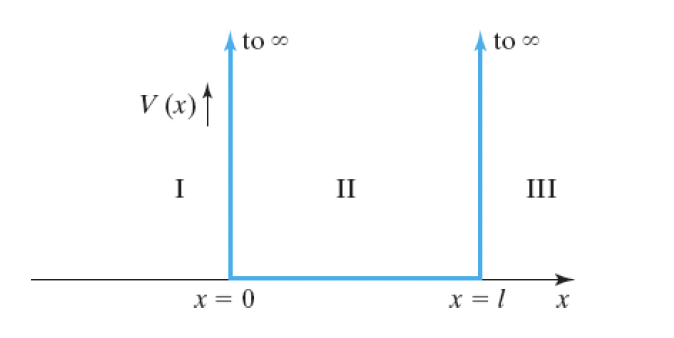
\includegraphics[width=0.6\textwidth]{/users/administrator/desktop/repo/quantumchemistry/Figures/2.1.png}  % 图片路径
		\caption{\text{一维盒子中粒子的势函数}$\: V\left(x\right)$}
		\label{fig:2.1}
	\end{figure}
	\\
	\indent 我们需要考虑三个区域。在区域I和III中,势能$V$为无穷大,此处的定态薛定谔方程(\ref{eq:1.19 time-independent Schrödinger Equation})为
	\begin{equation*}
		-\frac{\hbar^2}{2m}\frac{\mathrm{d}^2\psi}{\mathrm{d}x^2} = \left(E - \infty\right)\psi
	\end{equation*}
	与$\infty$相比,$E$的大小可以忽略不计。我们略去$E$,有
	\begin{equation*}
		\frac{\mathrm{d}^2\psi}{\mathrm{d}x^2} = \infty \psi, \quad \psi = \frac{1}{\infty}\frac{\mathrm{d}^2\psi}{\mathrm{d}x^2}
	\end{equation*}
	因此,在盒子的外侧,$\psi$为零:
	\begin{equation}
		\psi_I=0, \quad \psi_{II} = 0
		\label{eq:2.9 psi outside the box}
	\end{equation}
	\indent 对于区域II,$x$在0和$l$之间时,势能$V$为零,定态薛定谔方程(\ref{eq:1.19 time-independent Schrödinger Equation})为
	\begin{equation}
		\frac{\mathrm{d}^2\psi_{II}}{\mathrm{d}x^2}+\frac{2m}{\hbar^2}E\psi_{II}=0
		\label{eq:2.10 schrödinger equation for particle between 0 and l}
	\end{equation}
	其中$m$是粒子的质量,$E$是能量。我们将方程(\ref{eq:2.10 schrödinger equation for particle between 0 and l})视为一个二阶常系数线性齐次微分方程。其特征方程由(\ref{eq:2.7 auxiliary equation})给出:
	\begin{equation*}
		s^2 + 2mE\hbar^{-2}=0
	\end{equation*}
	\begin{equation}
		s = \pm \left(-2mE\right)^{1/2}\hbar^{-1}
		\label{eq:2.11}
	\end{equation}
	\begin{equation}
		s = \pm \mathrm{i}\left(2mE\right)^{1/2}\hbar^{-1}
		\label{eq:2.12}
	\end{equation}
	其中$\mathrm{i}$是虚数单位。使用(\ref{eq:2.8 general solution for 2.6}),我们有
	\begin{equation}
		\psi_{II} = c_1\mathrm{e}^{\mathrm{i} \left(2mE\right)^{1/2} x /\hbar}+c_2\mathrm{e}^{-\mathrm{i} \left(2mE\right)^{1/2} x /\hbar}
		\label{eq:2.13 general solution for particle between zero and l}
	\end{equation}
	我们姑且令
	\begin{equation*}
		\begin{aligned}
			\theta & \equiv \left(2mE\right)^{1/2} x /\hbar \\
			\psi_{II} & = c_1\mathrm{e}^{\mathrm{i}\theta}+c_1\mathrm{e}^{-\mathrm{i}\theta}
		\end{aligned}
	\end{equation*}
	由$\mathrm{e}^{\mathrm{i}\theta} = \cos\theta+\mathrm{i}\sin\theta$ $\left[\ref{eq:1.28 Euler's equation}\right]$以及
	\begin{equation}
		\boxed{
			\cos\left(-\theta\right) = \cos\theta \: \text{and} \: \sin\left(-\theta\right) = -\sin\theta
		}
		\label{eq:2.14 properties of sin and cos}
	\end{equation}
	我们有
	$\mathrm{e}^{-\mathrm{i}\theta} = \cos \left(-\theta\right)+\mathrm{i}\sin\left(-\theta\right)=\cos\theta-\mathrm{i}\sin\theta$
	。因此,
	\begin{equation*}
		\begin{aligned}
			\psi_{II} & =c_1\cos\theta+\mathrm{i}c_1\sin\theta+c_2\cos\theta-\mathrm{i}c_2\sin\theta \\
			& = \left(c_1+c_2\right)\cos\theta+\left(\mathrm{i}c_1-\mathrm{i}c_2\right)\sin\theta \\
			& = A \cos\theta + B\sin\theta 
		\end{aligned}	
	\end{equation*}
	其中,$A$和$B$是新的任意常数。则
	\begin{equation}
		\psi_{II}= A \cos\left[\hbar^{-1}\left(2mE\right)^{1/2}x\right]+B \sin\left[\hbar^{-1}\left(2mE\right)^{1/2}x\right]
		\label{eq:2.15 complete wave function of psi ii}
	\end{equation}
	\indent 现在通过定解条件,我们来求出$A$和$B$。假设波函数是连续的,也就是说,它的值不会突然跳变,这似乎是合理的(见图 3.4)。如果$\psi$在$x=0$处连续,那么有$\psi_I$和$\psi_{II}$在$x=0$处的极限相同:
	\begin{equation*}
		\begin{aligned}
			\lim\limits_{x \to 0}\psi_I & = \lim\limits_{x \to 0}\psi_{II} \\
			0 & = \lim\limits_{x \to 0}\left\{A \cos\left[\hbar^{-1}\left(2mE\right)^{1/2}x\right]+B \sin\left[\hbar^{-1}\left(2mE\right)^{1/2}x\right]\right\} \\
			0 & = A
		\end{aligned}
	\end{equation*}
	由于
	\begin{equation}
		\boxed{
			\sin 0 = 0, \quad \cos 0 =1
		}
		\label{eq:2.16 sin0 and cos0}
	\end{equation}
	将$A=0$带入(\ref{eq:2.15 complete wave function of psi ii}),有
	\begin{equation}
		\psi_{II} = B\sin\left[\left(2\pi/h\right)\left(2mE\right)^{1/2}x\right]
		\label{eq:2.17 }
	\end{equation}
	又由函数在$x=l$处连续,我们有
	\begin{equation}
		B\sin\left[\left(2\pi/h\right)\left(2mE\right)^{1/2}l\right]=0
		\label{eq:2.18}
	\end{equation}
	因为我们不能令波函数处处为零-得到一个空箱子,所以$B$不能为零。有
	\begin{equation*}
		\sin\left[\left(2\pi/h\right)\left(2mE\right)^{1/2}l\right]=0
	\end{equation*}
	$\sin$函数的零点位于$0, \pm \pi, \pm 2\pi, \cdots, \pm n \pi$。则
	\begin{equation}
		\left(2\pi/h\right)\left(2mE\right)^{1/2}l = \pm n \pi
		\label{eq:2.19 introduction of n}
	\end{equation}
	\indent $n=0$是一种特殊情况。由(\ref{eq:2.19 introduction of n}),$n=0$意味着$E=0$。若$E=0$则特征方程(\ref{eq:2.12})有两个相等的根,且式(\ref{eq:2.13 general solution for particle between zero and l})不是薛定谔方程的完全解。为了找到完全解,我们回到(\ref{eq:2.10 schrödinger equation for particle between 0 and l}),其中$E=0$有$frac{\mathrm{d}^2\psi_{II}}{\mathrm{d}x^2}=0$。积分一次,有$\mathrm{d}\psi_{II}/\mathrm{d}x = c$;再积分一次,有$\psi_{II}=cx+d$,其中$c$和$d$都是常数。由于$x=0$时有$\psi_{II}=0$,所以$d=0$;又由于$x=l$时也有$\psi_{II}=0$,所以$c=0$。因此,$\psi_{II}=0$推出$E=0$,则$E=0$不是允许的能量值。即$n=0$是不允许的。\\
	\indent 从方程(\ref{eq:2.19 introduction of n})中解出$E$,我们有
	\begin{equation}
		\boxed{
			E = \frac{n^2h^2}{8ml^2}, \quad n = 1,2,3 \cdots
		}
		\label{eq:2.20 energy of one-dimensional box}
	\end{equation}
	\indent 只有能量值满足式(\ref{eq:2.20 energy of one-dimensional box})的波函数$\psi$,才能符合在$x=l$处连续的定解条件。定解条件的应用迫使我们得出能量值是量子化的结论(图 2.2)。这与经典结果形成了鲜明对比,经典结果认为盒子中的粒子可以具有任何非负能量。请注意:粒子的能量有一个大于零的最小值。能量最小的状态称为\textbf{基态}。能量高于基态能量的状态为\textbf{激发态}。(在经典力学中,粒子在盒子中的最低能量为零。经典粒子在盒内静止不动时,动能为零,势能为零)。
	\begin{figure}[h!]
		\centering
		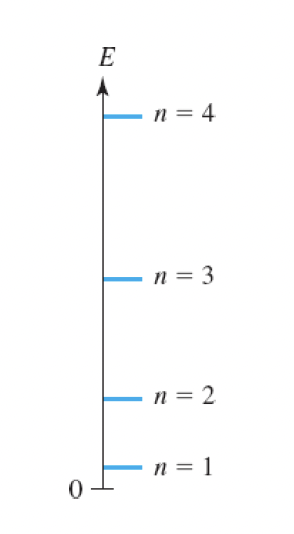
\includegraphics[width=0.2\textwidth]{/users/administrator/desktop/repo/quantumchemistry/Figures/2.2.png}  % 图片路径
		\caption{\text{一维盒子中粒子能量最低的四个能级}}
		\label{fig:2.2}
	\end{figure}
	\\
	\textbf{例题:}\\
	有一质量为$2.00\times10^{-26}\: \mathrm{g}$的粒子在长度$4.00 \: \mathrm{nm}$的势箱中运动。求该粒子从 $n=3$ 能级进入 $n=2$ 能级时发射光子的频率和波长。\\
	\indent 根据能量守恒,发射光子的能量等于两个定态之间的能量差[公式 (\ref{eq:1.4 Higher state to lower state delta energy}) ;另见第 9.9 节 ]:
	\begin{equation*}
		h\nu = E_{upper}-E_{lower}=\frac{n_u^2h^2}{8ml^2} - \frac{n_l^2h^2}{8ml^2}
	\end{equation*}
	\begin{equation*}
		\nu = \frac{\left(n_u^2-n_l^2\right)h}{8ml^2} = \frac{\left(3^2-2^2\right)\left(6.626 \times 10^{-34} \: \mathrm{J}\cdot\mathrm{s}\right)}{8\left(2.00 \times 10^{-29} \:  \mathrm{kg}\right)\left(4.00 \times 10^{-9} \: \mathrm{m}\right)^2} = 1.29 \times 10^{12} \: \mathrm{s}^{-1}
	\end{equation*}
	其中$u$和$l$分别代表高能级和低能级。由$\lambda \nu =c$,有$\lambda = 2.32 \times 10^{-4} \: \mathrm{m}$。(学生常见的错误是将 $h\nu$ 设为其中一个状态的能量,而不是状态间的能量\textit{差})\\
	\textbf{练习:}\\
	对于某个在一维盒子中运动的电子,其能级跃迁的最长波长为400 nm。求盒子的长度。\\
	\textit{答案:}0.603 nm\\
	
	\indent 将(\ref{eq:2.19 introduction of n})带入(\ref{eq:2.17 }),解出波函数为
	\begin{equation}
		\psi_{II} = B\sin\left(\frac{n\pi x}{l}\right), \quad n = 1,2,3\cdots
		\label{eq:2.21 wavefunction solution of psi ii with b}
	\end{equation}
	在 $n\pi$ 前面使用负号并不能得到另一个独立的解。因为 $\sin\left(-\theta\right)=-\sin\theta$,我们只会得到一个常数 -1,乘以带正号的解。\\
	\indent 公式 (\ref{eq:2.21 wavefunction solution of psi ii with b}) 中的常数 $B$ 仍然是任意的。为了将其确定下来,我们使用公式 (\ref{eq:1.24 the definition of nomalization}) 和 (\ref{eq:1.22 Psi and psi}) 对$\psi_{II}$进行归一化:
	\begin{equation*}
		\int_{-\infty}^{\infty}\left|\Psi\right|^2\mathrm{d}x = \int_{-\infty}^{\infty}\left|\psi\right|^2\mathrm{d}x = 1
	\end{equation*}
	\begin{equation*}
		\int_{-\infty}^{0}\left|\psi_I\right|^2\mathrm{d}x + \int_{0}^{l}\left|\psi_{II}\right|^2\mathrm{d}x +\int_{l}^{\infty}\left|\psi_{III}\right|^2\mathrm{d}x =1
	\end{equation*}
	\begin{equation}
		\left|B\right|^2\int_{0}^{l}\sin^2\left(\frac{n\pi x}{l}\right)\mathrm{d}x=1=\left|B\right|^2\frac{l}{2}
		\label{eq:2.22 process of fix constant B}
	\end{equation}
	其中的积分是用附录中的公式 (A.2) 求得的。我们有
	\begin{equation*}
		\left|B\right|^2=\left(2/l\right)^{1/2}
	\end{equation*}
	\indent 注意我们只求出了$B$的绝对值,但$B$可以取$\pm \left( 2/l\right) ^{1/2}$。此外,$B$也不必是实数,我们可以取任何模为$\left(2/l\right)^{1/2}$的复数。所以,我们可以说$B=\left( 2/l\right) ^{1/2}\mathrm{e}^{\mathrm{i}\alpha}$,其中$\alpha$是$B$的辐角,可以取0到$2\pi$之间的任何值(第 1.7 节)。取辐角为0,则箱中粒子的定态波函数为
	\begin{equation}
		\boxed{
			\psi_{II} = \left(\frac{2}{l}\right)^{1/2}\sin\left(\frac{n\pi x}{l}\right), \quad n = 1,2,3\cdots
		}
		\label{eq:2.23 stationary state wave function for the particle in a box}
	\end{equation}
	波函数和概率密度的图如图 \ref{fig:2.3} 和 \ref{fig:2.4} 所示。\\
	\indent 能量(\ref{eq:2.20 energy of one-dimensional box})和波函数(\ref{eq:2.23 stationary state wave function for the particle in a box})中的数字 $n$ 称为\textbf{量子数}。量子数 $n$ 的每个不同值都会产生不同的波函数和不同的状态。\\
	\indent 波函数在某些点为零,这些点被称为\textbf{节点}。量子数$n$每增加1,波函数$\psi$就多一个节点。$\psi$和$\left| \psi \right| ^2$ 中节点的存在似乎令人惊讶。因此,图(\ref{fig:2.4})表明:对于$n=2$,在箱的中点$x=2/l$处找到粒子的概率为零。粒子怎么可能从盒子的一侧运动到另一侧,而在任何时候都不会出现在盒子的中心呢?这个明显的悖论产生于我们试图用宏观粒子运动的日常经验来理解微观粒子的运动。然而,正如第 1 章所指出的:电子和其他微观 “粒子 ”无法用宏观世界的经典物理学概念来完整、正确地描述。\\
	\indent 图 \ref{fig:2.4} 显示,在盒子的不同位置找到粒子的概率与经典结果截然不同。从经典角度看,一个固定能量的粒子在盒子中以恒定的速度在两壁之间弹性地来回弹跳。因此,在盒子中的任何一点发现它的可能性都是相同的;从量子力学角度看,我们会发现在盒子中心的最低能级出现概率最大。随着能级越来越高,节点越来越多,概率的最大值和最小值就会越来越接近,而沿着盒子长度方向的概率变化最终会变得难以察觉。当量子数非常大时,我们就获得了接近于经典的均匀概率密度结果。
	\begin{figure}
		\centering
		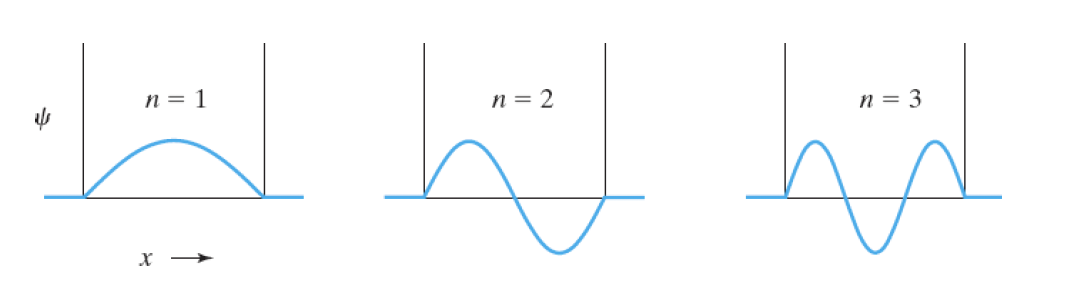
\includegraphics[width=0.8\textwidth]{/users/administrator/desktop/repo/quantumchemistry/Figures/2.3.png}  % 图片路径
		\caption{\text{三种能量最低的盒中粒子状态的} $\psi$ \text{曲线图}}
		\label{fig:2.3}
	\end{figure}
	\begin{figure}
		\centering
		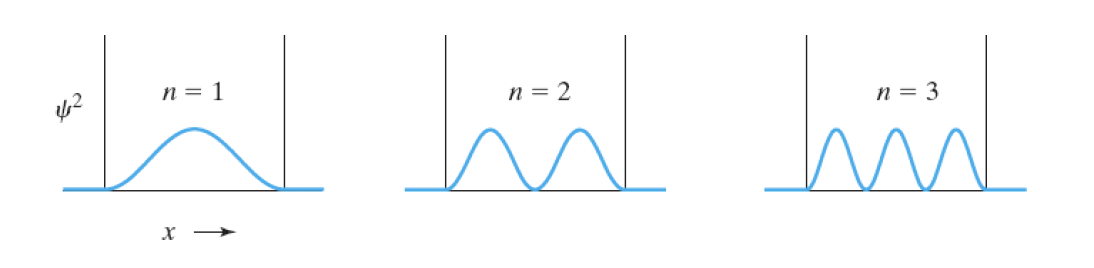
\includegraphics[width=0.8\textwidth]{/users/administrator/desktop/repo/quantumchemistry/Figures/2.4.png}  % 图片路径
		\caption{{三种能量最低的盒中粒子状态的} $\left| \psi \right| ^2$ \text{曲线图}}
		\label{fig:2.4}
	\end{figure}
	\indent 这一结果,即在大量子数极限下量子力学与经典力学的关系,被称为\textit{玻尔对应原理}。由于牛顿力学适用于宏观物体(运动速度远小于光速),我们期望非相对论量子力学能给出与经典力学对宏观物体相同的答案。由于普朗克常数极其微小,能量的量子化对于宏观物体来说是不可观测的。由于粒子的质量和盒子长度的平方出现在式 (\ref{eq:2.20 energy of one-dimensional box}) 的分母中,因此在宏观盒子中具有宏观运动能量的宏观物体将具有巨大的 $n$ 值,那么根据对应原理,宏观物体将显示出经典行为。\\
	\indent 现在,我们有了一整套波函数,每个波函数对应不同的能量,并以量子数 $n$(正整数)为特征。让下标 $i$ 表示量子数为 $n_i$ 的特定波函数:
	\begin{equation*}
			\psi_i = \left(\frac{2}{l}\right)^{1/2} \sin\left(\frac{n_i\pi x}{l}\right), \quad  0<x<l
	\end{equation*}
	\begin{equation*}
		\psi_i = 0, \quad  \text{其他区域}
	\end{equation*}
	由于波函数已归一化,我们有
	\begin{equation}
		\int_{-\infty}^{\infty}\psi_i^{\ast} \psi_j \mathrm{d}x = 1, \quad \text{若}i=j
		\label{eq:2.24}
	\end{equation}
	现在我们想知道,当我们使用对应于不同能级的波函数时,这个积分的值是多少:
	\begin{equation*}
		\int_{-\infty}^{\infty}\psi_i^{\ast} \psi_j \mathrm{d}x = \int_{0}^{l}\left(\frac{2}{l}\right)^{1/2}\sin\left(\frac{n_i\pi x}{l}\right)\left(\frac{2}{l}\right)^{1/2}\sin\left(\frac{n_j\pi x}{l}\right)\mathrm{d}x, \quad n_i \neq n_j
	\end{equation*}
	使用附录中的公式(A.5),我们有
	\begin{equation}
		\int_{-\infty}^{\infty}\psi_i^{\ast} \psi_j \mathrm{d}x = \frac{2}{l}\left[
			\frac{\sin \left[\left(n_i-n_j\right)\pi\right]}{2\left(n_i-n_j\right)\pi /l}- \frac{\sin \left[\left(n_i+n_j\right)\pi\right]}{2\left(n_i+n_j\right)\pi /l}
		\right] = 0
		\label{eq:2.25}
	\end{equation}
	由于当$m$是整数时有$\sin m \pi = 0$,则
	\begin{equation}
		\int_{-\infty}^{\infty}\psi_i^{\ast} \psi_j \mathrm{d}x = 0, \quad i \neq j
		\label{eq:2.26 definition of orthogonal wave functions}
	\end{equation}
	当(\ref{eq:2.26 definition of orthogonal wave functions})成立时,我们说对$i \neq j$的波函数$\psi_i$和$\psi_j$是互相\textbf{正交}的。将(\ref{eq:2.24})与(\ref{eq:2.26 definition of orthogonal wave functions})相结合,我们有
	\begin{equation}
		\int_{-\infty}^{\infty}\psi_i^{\ast} \psi_j \mathrm{d}x = \delta_{ij}
		\label{eq:2.27 orthogonal with kronecker delta}
	\end{equation}
	其中$\delta_{ij}$是\textbf{Kronecker符号}(由数学家的名字命名)。当$ $i 和 $j$ 相等时,它等于 1;当 $i$ 和 $j$ 不相等时,它等于 0:
	\begin{equation}
		\boxed{
			\delta_{ij} \equiv \begin{cases}
				0, \quad & i \neq j; \\
				1, \quad & i = j.
			\end{cases}
		}
		\label{eq:2.28 definition of kronecker delta}
	\end{equation}
	波函数的特性 (\ref{eq:2.27 orthogonal with kronecker delta})) 称为\textbf{正交归一性}。我们只证明了粒子盒内波函数的正交归一性。我们将在第 7.2 节更广泛地证明它。\\
	\indent 您可能会对式 (\ref{eq:2.26 definition of orthogonal wave functions}) 感到困惑,不明白为什么我们要将一个状态的波函数乘以另一个状态的波函数。我们稍后会看到(例如第 7.3 节),使用包含一个系统所有波函数之和的方程通常很有帮助,而这样的方程会导致像 (\ref{eq:2.26 definition of orthogonal wave functions}) 这样的积分。\\
	\indent 研究无限深势阱中粒子的一个更严谨的方法是:首先处理粒子在壁箱中的势能有限跃迁,然后当 $V$ 的跃迁变得无限大时求取极限。取极限时的结果与 (\ref{eq:2.20 energy of one-dimensional box}) 和 (\ref{eq:2.23 stationary state wave function for the particle in a box}) 相同(见问题 2.22)。\\
	\indent 我们只考虑了粒子在一维盒子中的定态。该系统的非稳态示例,请参见第 7.8 节末尾的示例。\\
	\indent 关于粒子在盒子中的在线计算机模拟,请访问 www.chem.uci.edu/undergraduate/applets/dwell/\\dwell.htm(显示了在盒子中间引入高度和宽度可变的屏障时对波函数和能级的影响);web. williams.\\edu/wpetc/chemistry/dbingemann/Chem153/particle.html(通过绘制薛定谔方程在能量变化和盒子长度变化时的解来显示量子化);以及 falstad.com/qm1d/(同时显示含时薛定谔方程和定态薛定谔方程;见 7.47)。






\section{一维自由粒子}

\section{矩形势井中的粒子}

\section{隧穿}

\section*{总结}

\section*{习题}
